\documentclass[14pt, final,numbered]{ifacconf}
\usepackage{caption}
\pagestyle{plain}           % Default for rest of the pages
\pagenumbering{arabic}      % Arabic numerals
\maketitle
\thispagestyle{plain}  
\usepackage[strings]{underscore}


\usepackage{graphicx}
\usepackage{natbib}
\usepackage{amsmath}
\usepackage{amsfonts}
\usepackage{booktabs}
\usepackage[compatibility=false]{caption}
\captionsetup[table]{font=Large, labelfont=bf, justification=centering}
\usepackage{float}
\usepackage{tcolorbox}
\usepackage{adjustbox}

\begin{document}

\begin{frontmatter}

\title{Evaluating the Economic Feasibility of Residential Solar and Battery Colocation: A Cost Optimization Approach}


\author{Xinyu Luo}
\address{Institute for Computing in Research}

\author{Sung Bum Ahn}
\address{Electric Reliability Council of Texas, Taylor TX}

\begin{abstract}
Residential solar and battery colocation can reduce household electricity costs by storing excess solar energy for later use and reducing electricity purchases during high-priced periods. This study aims to examine the optimal battery size for PV-battery systems in the San Diego area by creating a model that optimizes battery dispatch across a range of battery capacities for summer and winter months. The model employs hourly residential load profiles, solar generation profiles, time-of-use-pricing, and export credit rates to determine the battery capacity that minimizes electricity purchase costs and balances the tradeoff between operational savings and annualized capital cost. The results indicate that the economically optimal battery capacity is 12 kWh during the summer and 10 kWh during the winter. The larger optimal battery in summer is driven by greater solar energy production, which provides more excess electricity for storage and increases opportunities to reduce purchases during high-priced periods. In contrast, lower winter solar generation and electricity prices reduces the economic benefit of additional storage, making a smaller battery more cost-effective. These findings show that optimal battery size varies with seasonal solar generation and household electricity demand, highlighting the importance of season-specific analysis when sizing residential PV-battery storage systems.
\end{abstract}

\end{frontmatter}
\section{Introduction}
Renewable energy has become an increasingly viable option for homeowners in recent years due to rising electricity prices, power outages, and concerns about carbon emissions from fossil fuels. Through residential renewable energy systems, homeowners are less dependent on large external power grids and are less vulnerable to price hikes in traditional utility rates. Federal and state incentives, such as investment tax credits (ITC) and cash rebates, have also widely supported this transition to renewable energy. 

Residential solar systems generally use photovoltaic (PV) technology to generate solar power, where photovoltaic cells in solar panels convert solar radiation directly into electricity \cite{bagalini2019solar}. These cells, typically made of silicon, contain layers with different electrical properties that create an electric field when struck by sunlight. This process knocks electrons loose and generates a flow of direct current (DC) electricity. Since most homes run on alternating current (AC), an inverter is used to convert DC electricity into usable AC power for household appliances. Solar power follows a predictable generation pattern, unlike other forms of renewable energy, with electricity produced only during daylight hours. However, this leads to a misalignment between peak production and consumption periods, as residential energy demand often peaks in the early morning and evening when solar generation is minimal. Thus, battery energy storage systems can be combined with solar to store excess energy generated throughout the day, and discharge during periods of high demand \cite{scanu2024solar}. With demand for renewable energy increasing globally, co-locating battery storage with solar PV appears as a versatile solution to meet the needs of homeowners and grid operators. 

Co-location refers to the installation of a residential battery storage alongside a rooftop PV system, and is often referred to as a PV-battery system \cite{scanu2024solar}. The two systems share a common grid connection and supporting electrical infrastructure, reducing costs and allowing for the battery to store excess solar generation for later use or export to the grid. Since local net metering policies credit homeowners for sending excess electricity generated through solar back to the grid, residential batteries can store excess solar generated throughout the day and export to the grid for credits. However in April of 2023, SDG\&E adopted NEM (Net Energy Metering) 3.0, which features a 75\% reduction in export rates (the value of excess electricity sent to the grid by solar systems) and ended net metering entirely. The policy reduces overall savings,and increases the payback period of residential solar for homeowners. It was designed to encourage homeowners to pair battery storage with their solar panels to become more self-sufficient. 

Sun et al. reviewed over 500,000 US households  and evaluated the economic and back-up viability of solar-battery systems \cite{sun2025solar}. They found that 60\% of American households could reduce electricity costs by an average of 15\%, and 63\% of them could achieve affordable back-up power during power outages that could cover an average of 51\% of their essential energy needs (Stanford paper). With the frequency extreme weather events growing due to climate change, battery storage provides a practical means of providing households with backup power during electricity outages. Baik et al. investigated the resilience value of these systems during blackouts, and found that the introduction of PV-battery systems can effectively mitigate expected load loss caused by electricity outages across all regions of the United States \cite{baik2024resilience} 

Additionally, Bollinger et al. examined the complementarities in the demand for rooftop solar and battery energy storage, and found that if storage were not available, over 20\% of households who co-adopt solar and storage would not adopt anything \cite{bollinger2023valuing}. 

Prior studies on the value of coupled renewable-battery plants compared to independent installations determined that coupling offers cost savings through lower electricity prices and the investment tax credit incentives, but also introduces operational and geographic constraints that can reduce the market value of the battery relative to independently sited systems. Gorman et al. demonstrated that coupling limits the potential locations of batteries, leading to the coupling penalty, or missed value from independently siting the battery in an optimal location away from solar plants \cite{gorman2022coupled}. However, their results suggested that the tradeoffs between coupling penalties and savings would vary by situation as a result of the wide regional variation in coupling penalties. 

Tervo et al. found that while an ITC provides money back in the first year of operation by reducing taxes owed, the long-term economic value of PV-battery systems depends on the state's electricity prices and incentives with high export prices \cite{tervo2018battery}.

A similar study examining residential PV–battery systems and their profitability has been conducted in China, where researchers found that these systems would not be economically viable due to the country's low electricity tariffs and PV generation incentives which do not take into account storage. They reported that doubling the electricity price and halving export tariffs would make the PV-battery investment profitable \cite{bagalini2019solar}. Currently, many regions in the United States employ time-of-use tariffs, or electricity pricing structures that vary depending on the time of day, day of the week, and season. The most expensive rates generally apply during high demand windows, such as the afternoon from 5:00 PM to 9:00 PM. 

Our work builds on this foundation of investigating the economic feasibility of residential PV-battery storage systems for homeowners in the United States by examining how battery storage capacity can be optimally sized during both the summer and winter months to minimize electricity costs under current time-of-use pricing while accounting for the battery's amortized capital cost. Incorporating battery ownership cost into the optimization enables the tradeoff between operational savings and additional storage capacity to be evaluated, allowing the economically optimal battery size to be identified.

San Diego, California, serves as a case study because of its high electricity prices, favorable solar resources, and widespread adoption of residential solar systems. The proposed cost model incorporates seasonal hourly residential load profiles, hourly PV generation, time-of-use electricity tariffs, and hourly export credits to determine the optimal battery storage size. The findings of this study contribute to a better understanding of how battery size, seasonal electricity demand, and time-of-use pricing influence homeowner savings. These results can help homeowners make more informed investment decisions and provide a framework for evaluating the economic viability of residential PV-battery systems in other regions with different electricity prices and solar resources.

\section{Methods and data}
This study combines publicly available datasets describing residential electricity demand, PV generation, time-of-use tariffs, and battery export compensation. Representative residential load profiles were obtained from the Open Energy Data Initiative's residential hourly load profiles, while hourly PV generation was generated using the National Renewable Energy Laboratory (NREL) PVWatts model. Time-of-use electricity tariffs and Net Billing Tariff (NBT) export prices for San Diego Gas \& Electric (SDG\&E) were used to represent the economic environment for residential PV customers. These four datasets and pricing policies were integrated in the cost-minimization model to examine which battery capacity would minimize total costs on weekdays for homeowners. Our study focuses on weekdays because time-of-use electricity pricing in San Diego are generally higher on weekdays than on weekends. Modeling weekday electricity consumption therefore captures periods when battery storage has the greatest potential to reduce electricity costs through load shifting.

\subsection{Residential Load Profiles}
The residential hourly load profiles were generated using Energy Plus, a building simulation that represents a single-family detached home constructed to the 2009 International Energy Conservation Code (IECC) and simulated using Typical Meteorological Year 3 (TMY3) weather data to estimate hourly residential electricity demand. This study uses the BASE case for the San Diego Miramar location, which provides hourly residential electricity demand over a representative one-year period. The hourly electricity demand values were obtained from the Electricity: Facility output, measured in kilowatt-hours (kWh). 

To reduce short-term fluctuations while preserving the overall daily demand pattern for the summer and winter seasons, we smoothed the hourly load profile using a Fast Fourier Transform (FFT) and compared it to averaging the load profiles. The FFT converts the time-domain load profile into its frequency-domain representation, decomposing the signal into a set of sinusoidal components, where each component represents a different frequency present in the original signal. Low-frequency components capture broad daily demand trends, while high-frequency components represent short-term fluctuations and noise. To smooth the load profile, only the mean value and the lowest-frequency Fourier coefficients were retained. Specifically, the first 500 harmonic pairs were preserved, while all remaining higher-frequency coefficients were set to zero. The frequency spectrum was then reconstructed in the time domain using the inverse Fast Fourier Transform (IFFT). The resulting smoothed load profile maintains the overall shape and daily demand characteristics of the original data while removing high-frequency fluctuations. 

Although FFT smoothing produced a continuous representation of the daily load profile, it also reduced the magnitude of the evening demand peak, which is a key feature influencing residential battery charging and discharging decisions. Because the objective of this study is to evaluate optimal battery operation under representative residential demand patterns, preserving these seasonal load characteristics was considered more important than smoothing short-term variability. Therefore, representative summer, winter, and annual load profiles were constructed by calculating the average electricity demand for each hour across all days within the corresponding season. The load profiles are displayed below, and later used in conjunction with the time-of-use tariffs in the cost optimization model. 
\begin{figure}[h]
    \centering
    
\includegraphics[width=0.5\textwidth]{san_diego_load_profiles.png}
    \caption{Representative seasonal Fourier-smoothed load profiles for San Diego Miramar region}
    \label{fig:load_image}
\end{figure}
\subsection{Solar Generation Profiles}
To obtain solar generation data for the same region, we used the National Renewable Energy Laboratory's (NREL) PVWatts® Version 8 calculator. PVWatts estimates the hourly electricity generation of a PV system based on system characteristics, geographic location, and historical weather data. The model was configured using the coordinates of the San Diego Miramar location, and hourly AC electricity generation data from the NLR's National Solar Radiation Database were obtained for a representative one-year period. The size of the PV system was set to 6 kW, representing the lower end of a typical residential rooftop installation since an average single-family home rooftop PV system ranges from 6 kW to 8 kW in size. This conservative assumption allowed the economic feasibility of residential PV-battery systems to be evaluated under less favorable solar generation conditions. The tilt of the solar panels was set to 25° and the azimuth angle was set to 180° due to San Diego's latitude and location in the Northern Hemisphere. The module type, array type, DC to AC ratio, ground coverage ratio, inverter efficiency, and system losses were set to the PVWatts default assumption values. The search radius for the closest climate data station was 100 miles. The solar generation data was split by season, specifically summer and winter, since the daily profiles differ greatly depending on day length and sun angle. For each season, the hourly generation values were averaged across all weekdays to produce representative 24-hour solar generation profiles. These representative profiles were then used as inputs for the PV system's generation ability in the battery optimization model.

\begin{figure}[h]
    \centering
    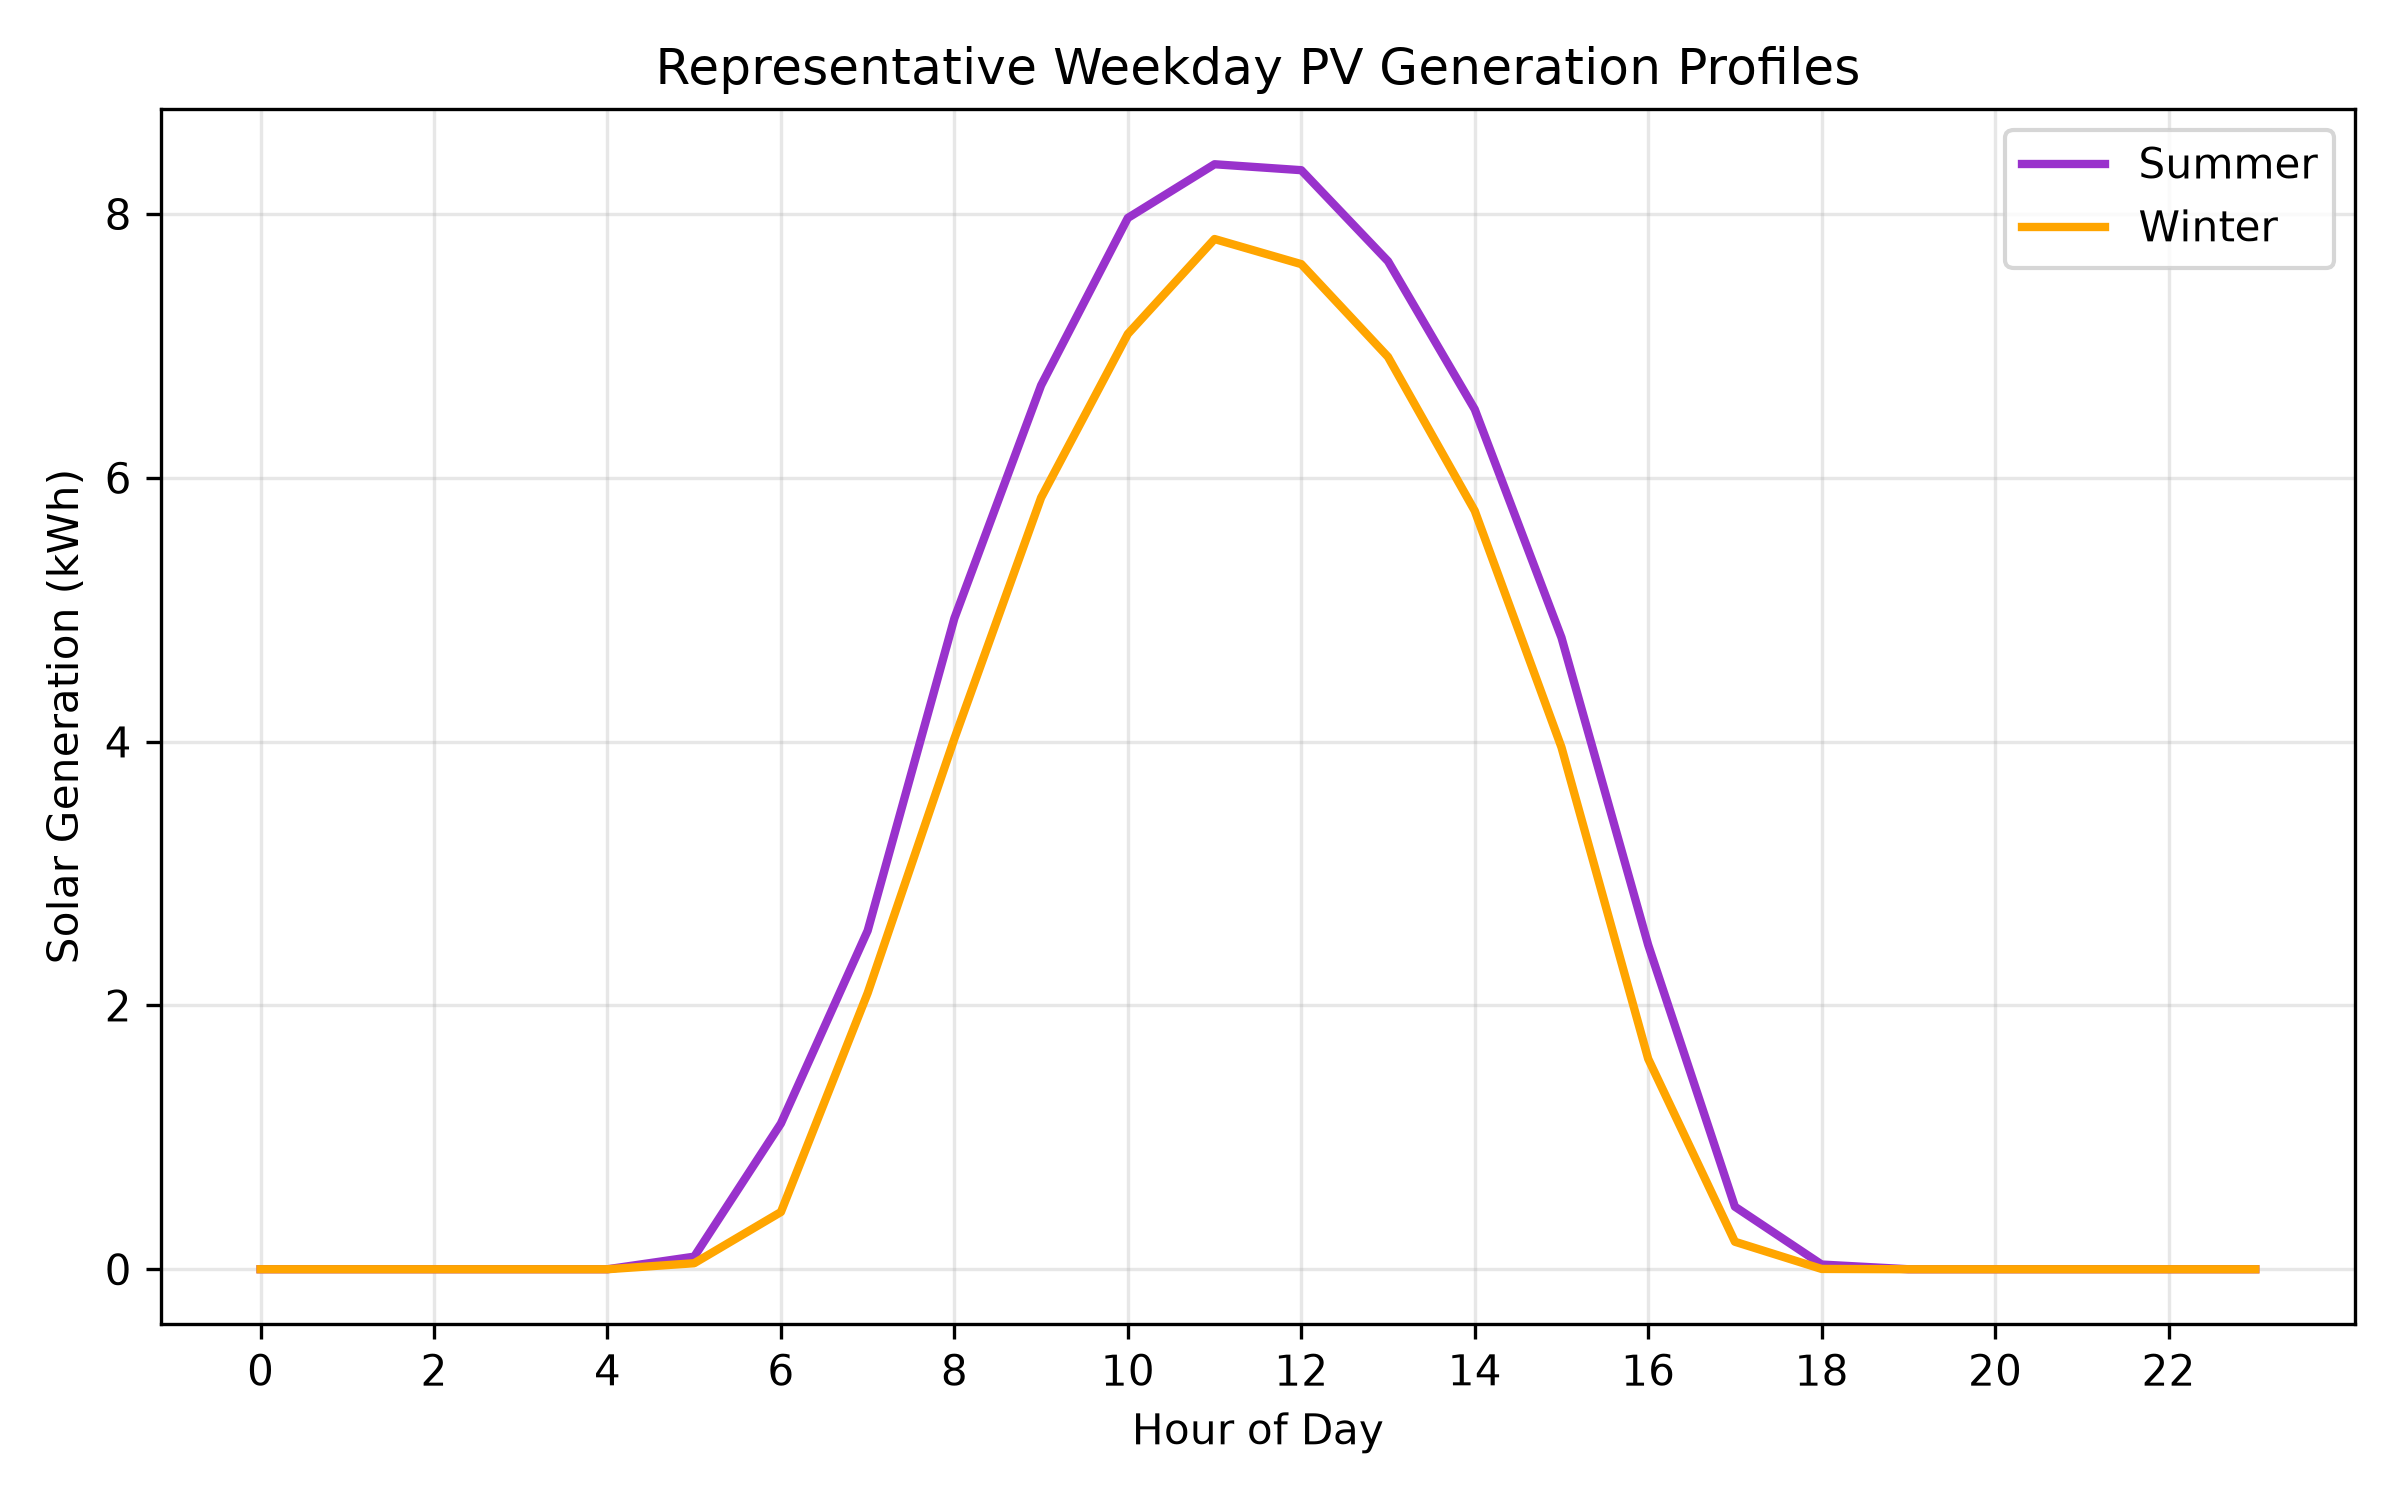
\includegraphics[width=0.5\textwidth]{seasonal_solar_profiles.png}
    \caption{Representative seasonal daily solar generation profiles for San Diego Miramar region}
    \label{fig:solar_image}
\end{figure}

\subsection{TOU Pricing}
The electric utility serving San Diego is San Diego Gas \& Electric (SDG\&E). Residential electricity rates are based on time-of-use (TOU) pricing, under which the price of electricity varies by time of day and day of the week. SDG\&E defines six TOU periods, each corresponding to a different electricity price. Only the prices for winter and summer months were used in the model alongside the residential load profiles to calculate for the cost of electricity without any kind of PV system. The following rates and charge schedule were found on the Open Energy Initiative's U.S. Utility Rate Database. 

\begin{table}[ht]
\centering
\begin{tabular}{|c|r|}
\hline
Period & Rate (\$/kWh) \\
\hline
1 & 0.71598 \\
2 & 0.38853 \\
3 & 0.34545 \\
4 & 0.50219 \\
5 & 0.37682 \\
6 & 0.33764 \\
\hline
\end{tabular}

\vspace{0.3cm}
\caption{Energy Usage Charge Structure (Entire Year)}
\label{tab:my_table}
\end{table}

\begin{figure}[h]
    \centering
    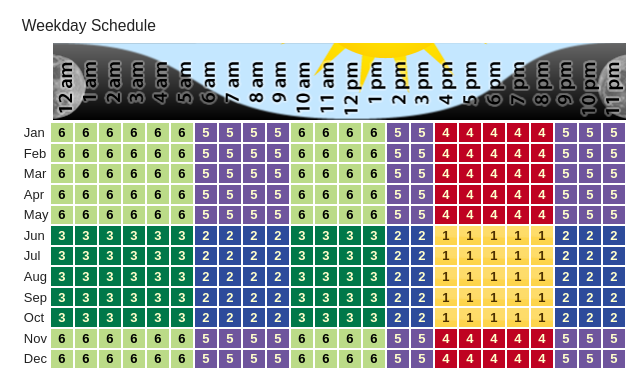
\includegraphics[width=0.25\textwidth]{tou_pricing.png}
    \caption{Residential Energy Usage Charge Schedule}
    \label{fig:tou_image}
\end{figure}

\subsection{Energy Export Credits}
The SDG\&E’s Solar Billing Plan provides Energy Export Credit rates for the first nine years following a customer’s system installation, with the applicable rates determined by the installation year. These credits are based on the California Public Utilities Commission’s Avoided Cost Calculator (ACC), which estimates the value of electricity exported to the grid according to the time of day and the utility costs avoided by that export. SDG\&E’s Solar Billing Plan provides energy export credit rates for the first nine years following a customer’s system installation, with the applicable rates determined by the installation year. These credits are based on the California Public Utilities Commission’s Avoided Cost Calculator (ACC), which estimates the value of electricity exported to the grid according to the time of day and the utility costs avoided by that export. For each hour and weekday, the total Energy Export Credit is calculated as the sum of the corresponding Generation and Delivery components. The Generation credit reflects the ACC's generation-side avoided costs, while the Delivery credit reflects avoided transmission and distribution costs associated with delivering electricity to customers.

We used the Current Year (2026) NBT Export Pricing file for the value of Energy Export Credits in our cost minimization model, and only examined the next nine years since the export credit rates are locked-in for the next nine years, and all rates for following years are simply for illustrative purposes. We calculated the export credit to be the sum of the Generation and Delivery Components by adding their values together. Then, we took the average Energy Export Credit rate by hour and year for both summer and winter to create the hourly export credit costs for our model. For the model, we averaged the export credit rates of this year and the next two years (2026-2028) by season, since our study focuses on the near-term economic feasibility of PV-battery systems, and how to optimize battery storage following current regulations. After 2028, the yearly export credit rates change drastically and have a much higher evening peak compared to previous years. 

\begin{figure}[h]
    \centering
    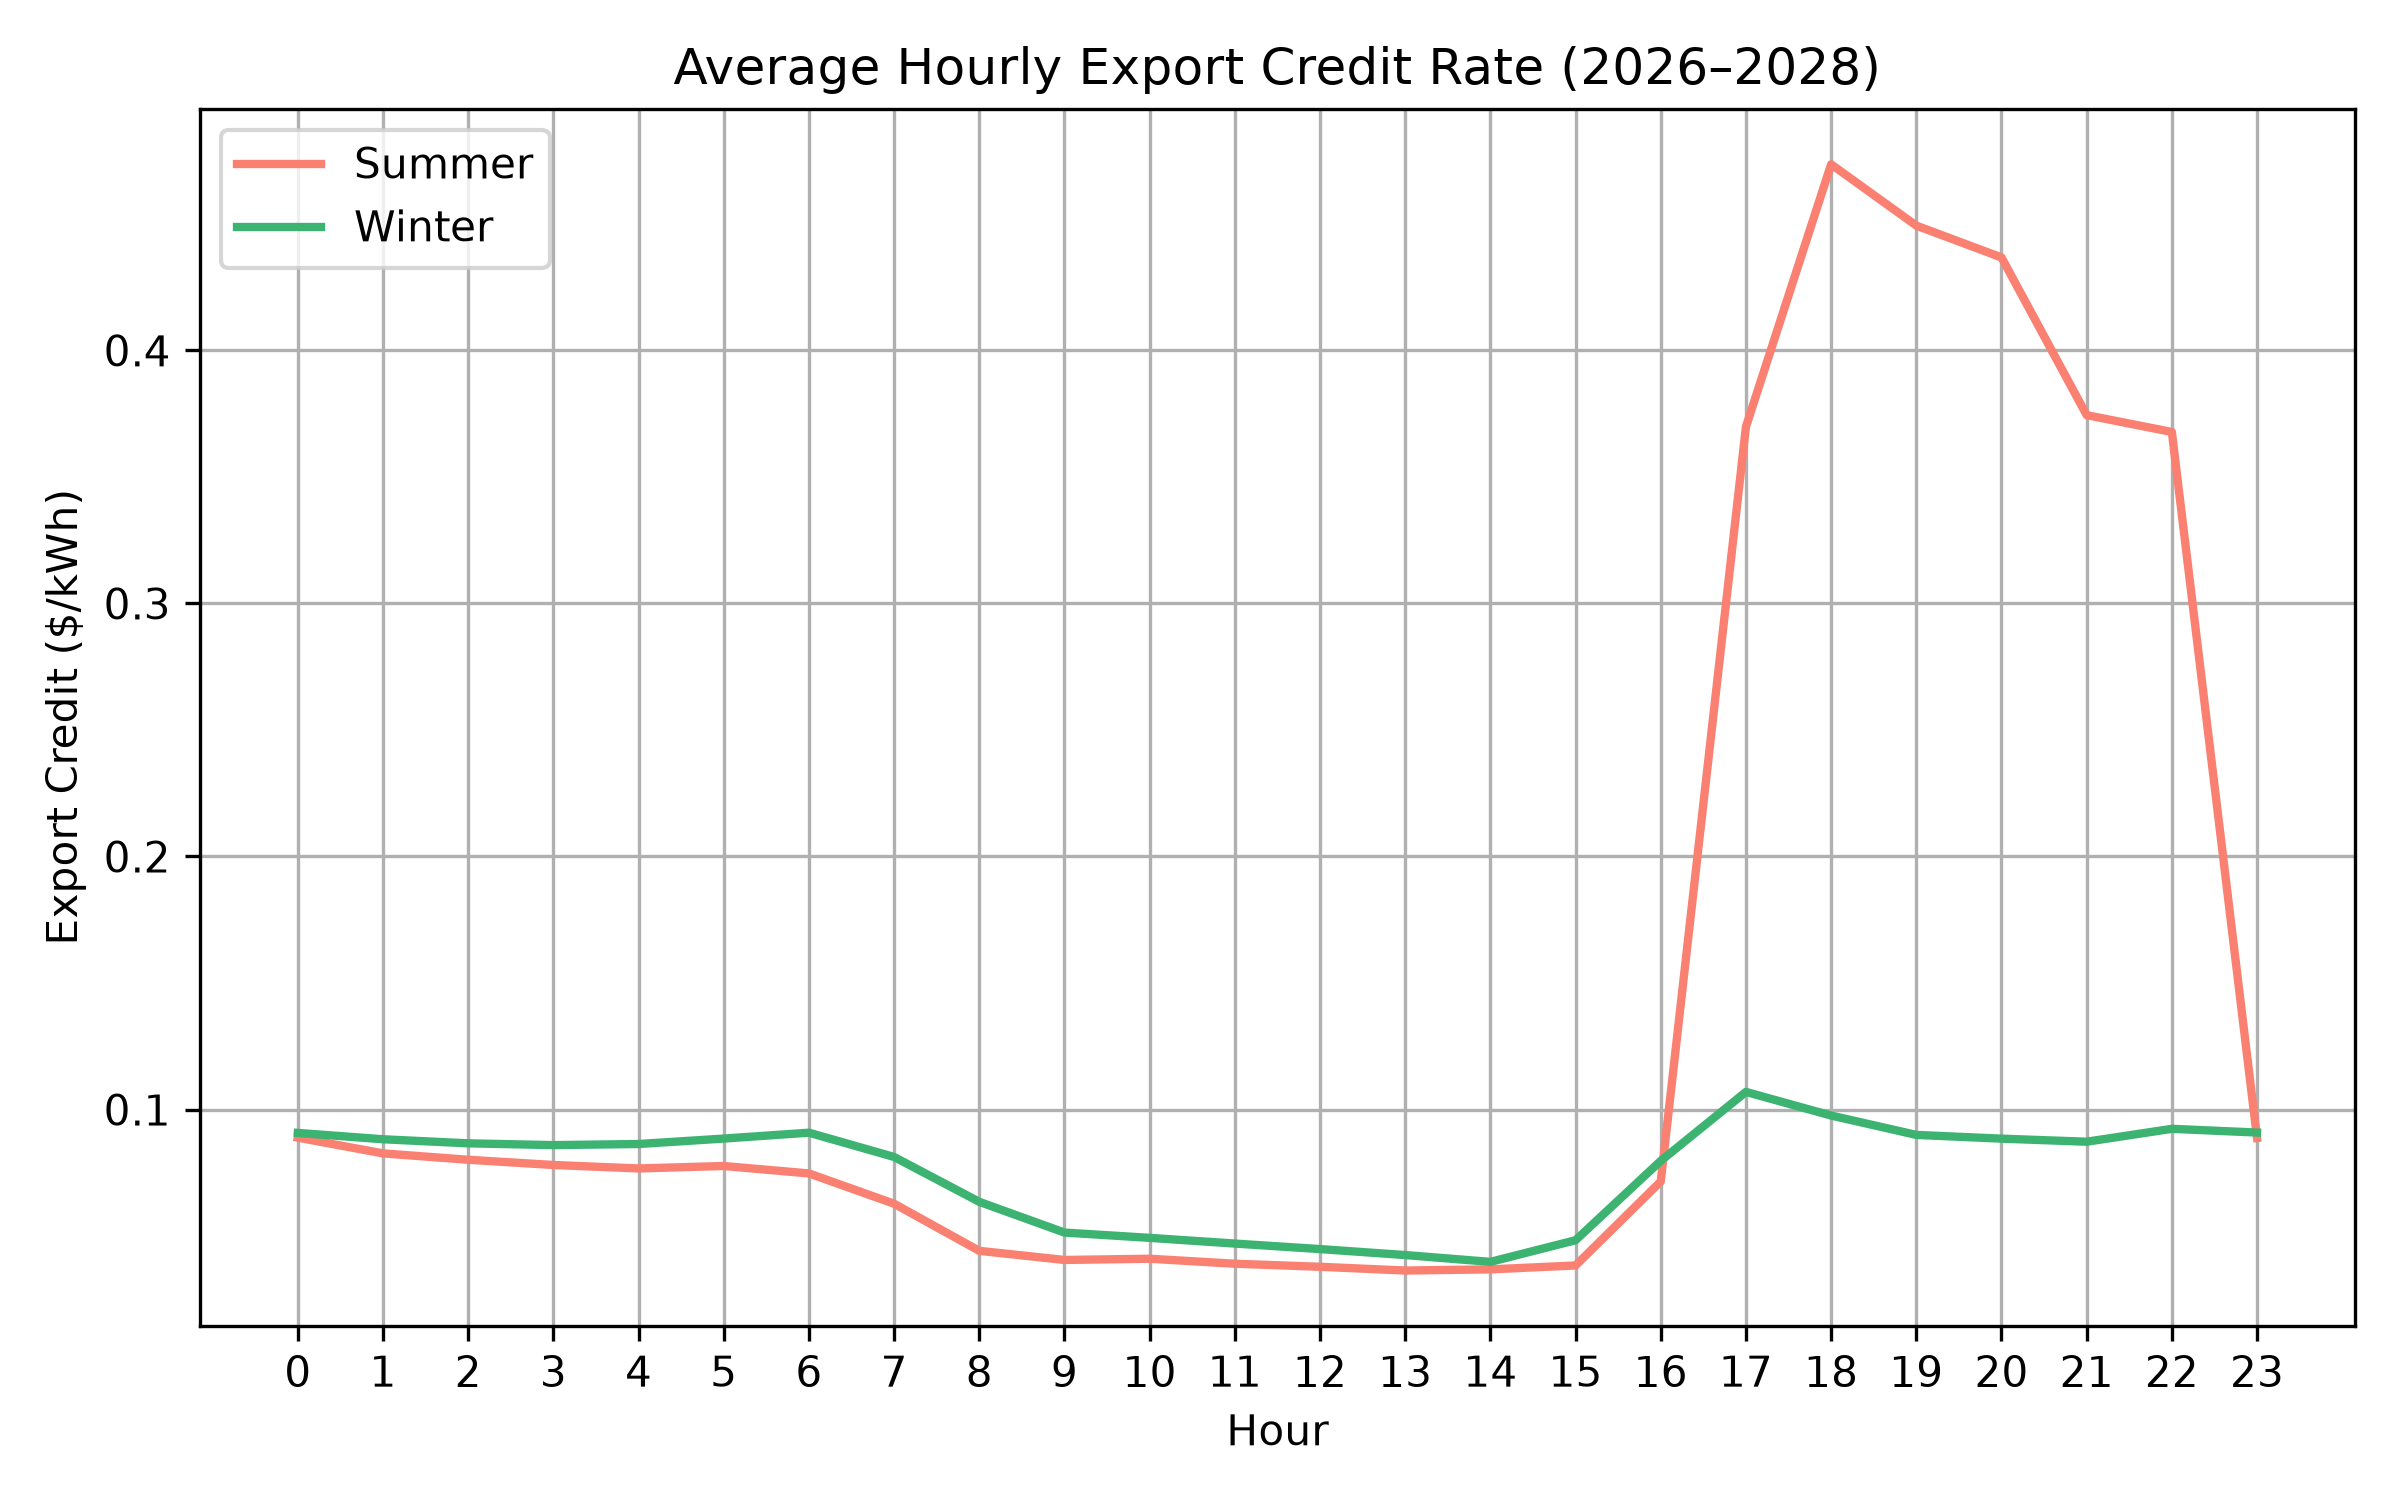
\includegraphics[width=0.5\textwidth]{export_profile_2026_2028.png}
    \caption{Export Credit Rates}
    \label{fig:exportprofiles_image}
\end{figure}

\subsection{Cost Minimization Model}
The cost minimization model aims to identify the battery capacity that minimizes the total cost of electricity and battery ownership for a residential PV-battery system under time-of-use pricing by optimizing battery dispatch across multiple battery sizes. The model uses the CVXPY Python optimization library to approach this cost optimization problem, along with the residential load profiles, solar generation profiles, export credit rates, and TOU pricing. The hourly load profiles were multiplied with the TOU pricing to calculate what the electricity costs for a household without any form of renewable energy would be. The optimization variables include the battery state of charge (SOC), grid electricity imports, grid electricity exports, battery charging from PV generation, and battery discharging to meet household electricity demand. The constraints included keeping the SOC within battery capacity limits, allowing the battery to only charge/discharge half of the battery's total capacity in an hour due to power limits,and forcing the battery to start and end the day at half its total capacity so the battery isn't completely emptied at night to reduce the day's bill and start empty the next day. Furthermore, the battery cannot directly charge from the grid, only from PV generation. The battery charging and discharging efficiencies are each assumed to be 95\%, consistent with typical values reported for residential lithium-ion battery systems. The energy balance constraint requires that, at every hour, electricity supplied by the PV system, the utility grid, and battery discharge equals the electricity consumed by the household load, battery charging, and grid exports.

\subsection{Amortized Capital Cost}
We also considered the battery's amortized capital cost, which spreads the upfront investment over the battery's expected lifetime, to evaluate the tradeoff between reduced electricity costs and the additional cost of larger battery capacities. The cost of battery storage was \$800 per kWh, which represents current residential lithium-ion battery costs. Fixed installation costs were not considered in this study because they do not depend on battery size. The discount rate accounts for the time value of money, and was set at 7\% and on par with the NREL's studies of solar PV systems. The model also assumes that all battery sizes remain in service for 10 years, consistent with the warranty period of many residential lithium-ion battery systems. A reduction of \$200/kWh for the incentives rate comes from California's Self-Generation Incentives Program (SGIP) which applies to owner-purchased systems. The battery's original upfront cost was calculated, and then the net cost considering federal incentives. San Diego's local incentives or rebates do not apply here, since the Single-family Affordable Solar Homes (SASH) solar rebates program is designed for low-income residents. The annualized capital cost was calculated using the net cost, and the Capital Recovery Factor (CRF) which converts the battery's upfront capital cost into an equivalent annual cost over its expected lifetime while accounting for the time value of money. This cost was divided by 365 to obtain the daily amortized battery cost used in the optimization model.

\begin{equation}
\mathrm{CRF} =
\frac{r(1+r)^n}{(1+r)^n-1},
\end{equation}

\begin{equation}
C_{\mathrm{annual}}
=
C_{\mathrm{net}}
\times
\mathrm{CRF},
\end{equation}

\subsection{Model Objective}
The optimization objective minimizes the combined daily electricity cost, which includes the costs of exporting to and importing from the grid. Including the annualized battery cost allows the model to balance reductions in electricity expenses against the additional cost of installing a larger battery. The optimization problem is defined using the objective function and the system constraints, and is then solved by CVXPY to determine the optimal battery dispatch strategy for each battery capacity. CVXPY produces tiny nonzero values because of numerical precision, so all values below 1e-6 were treated as zero. These results were compared to the no-battery case, where a PV system was in place with no battery storage, and the annualized battery cost is subtracted from the bill savings. The model was ran a total of seven times, at battery capacities (kWh) of 4, 6, 10, 12, 14, 16, and 20 for both summer and winter seasons. These capacities are spaced out and within the range of typical residential PV-battery system sizes. The battery capacity with the highest net benefit (bill savings minus annualized battery cost) was determined to be the best option for homeowners in San Diego. 

\section{Results}
Table 2 summarizes the results for the optimal battery in each season, including the optimal battery capacity, the daily operating cost after optimization, daily bill savings relative to the no-battery case, annualized battery capital cost, and the resulting daily and annual net benefits.

\begin{table}[H]
\centering
\caption{Optimal battery sizing results for the representative summer and winter profiles}
\label{tab:battery_results}
\begin{tabular}{lcc}
\toprule
\textbf{Metric} & \textbf{Summer} & \textbf{Winter} \\
\midrule
Optimal Battery Capacity (kWh) & 12 & 10 \\
Daily Operating Cost (\$) & -0.24 & 0.35 \\
Daily Bill Savings (\$) & 4.76 & 3.29 \\
Annualized Capital Cost (\$/yr) & 1025.12 & 854.27 \\
Daily Net Benefit (\$) & 1.95 & 0.95 \\
Annual Net Benefit (\$/yr) & 711.75 & 346.75 \\
\bottomrule
\end{tabular}
\end{table}

The results indicate that the economically optimal battery capacity differs by season. For the representative summer profile, a 12 kWh battery produced the highest net benefit of $1.95 per day ($711.75 per year), while a 10 kWh battery was optimal for the representative winter profile, yielding a net benefit of $0.95 per day ($346.75 per year). 

\subsection{Net benefit vs. battery size}
The figures below display the net benefit versus battery capacity curve, with the optimal battery size corresponding to the highest net benefit. 
\begin{figure}[h]
    \centering
    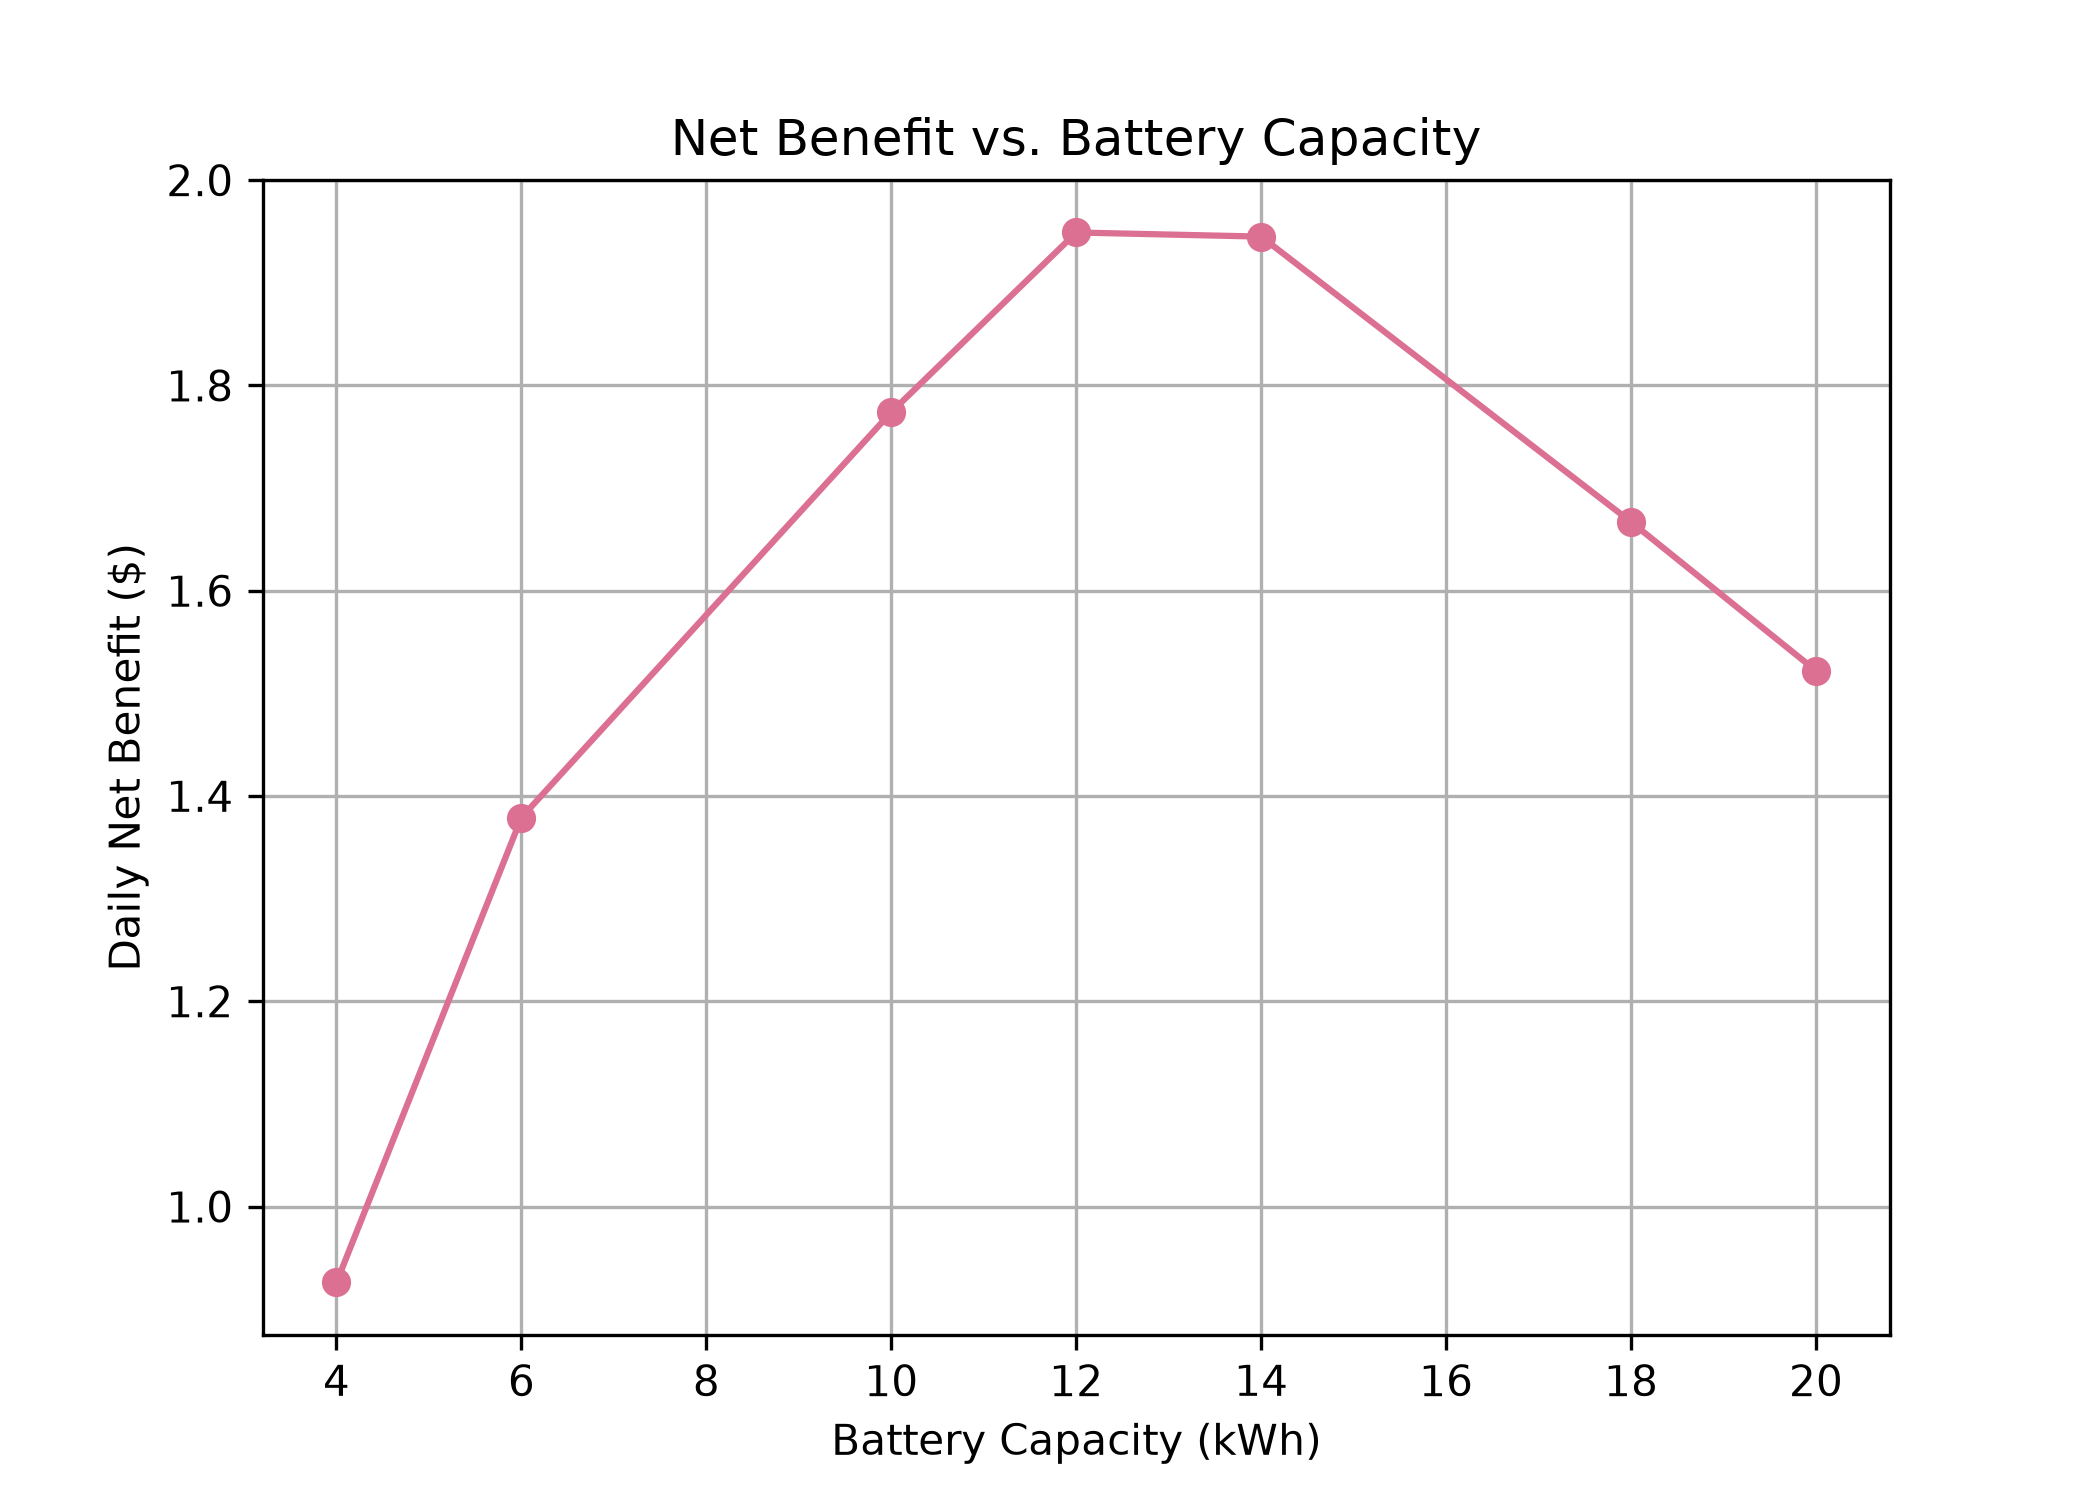
\includegraphics[width=0.5\textwidth]{summer_net_benefit_vs_capacity.png}
    \caption{Summer Net Benefit vs. Battery Capacity}
    \label{fig:summer_net_benefit_image}
\end{figure}

\begin{figure}[h]
    \centering
    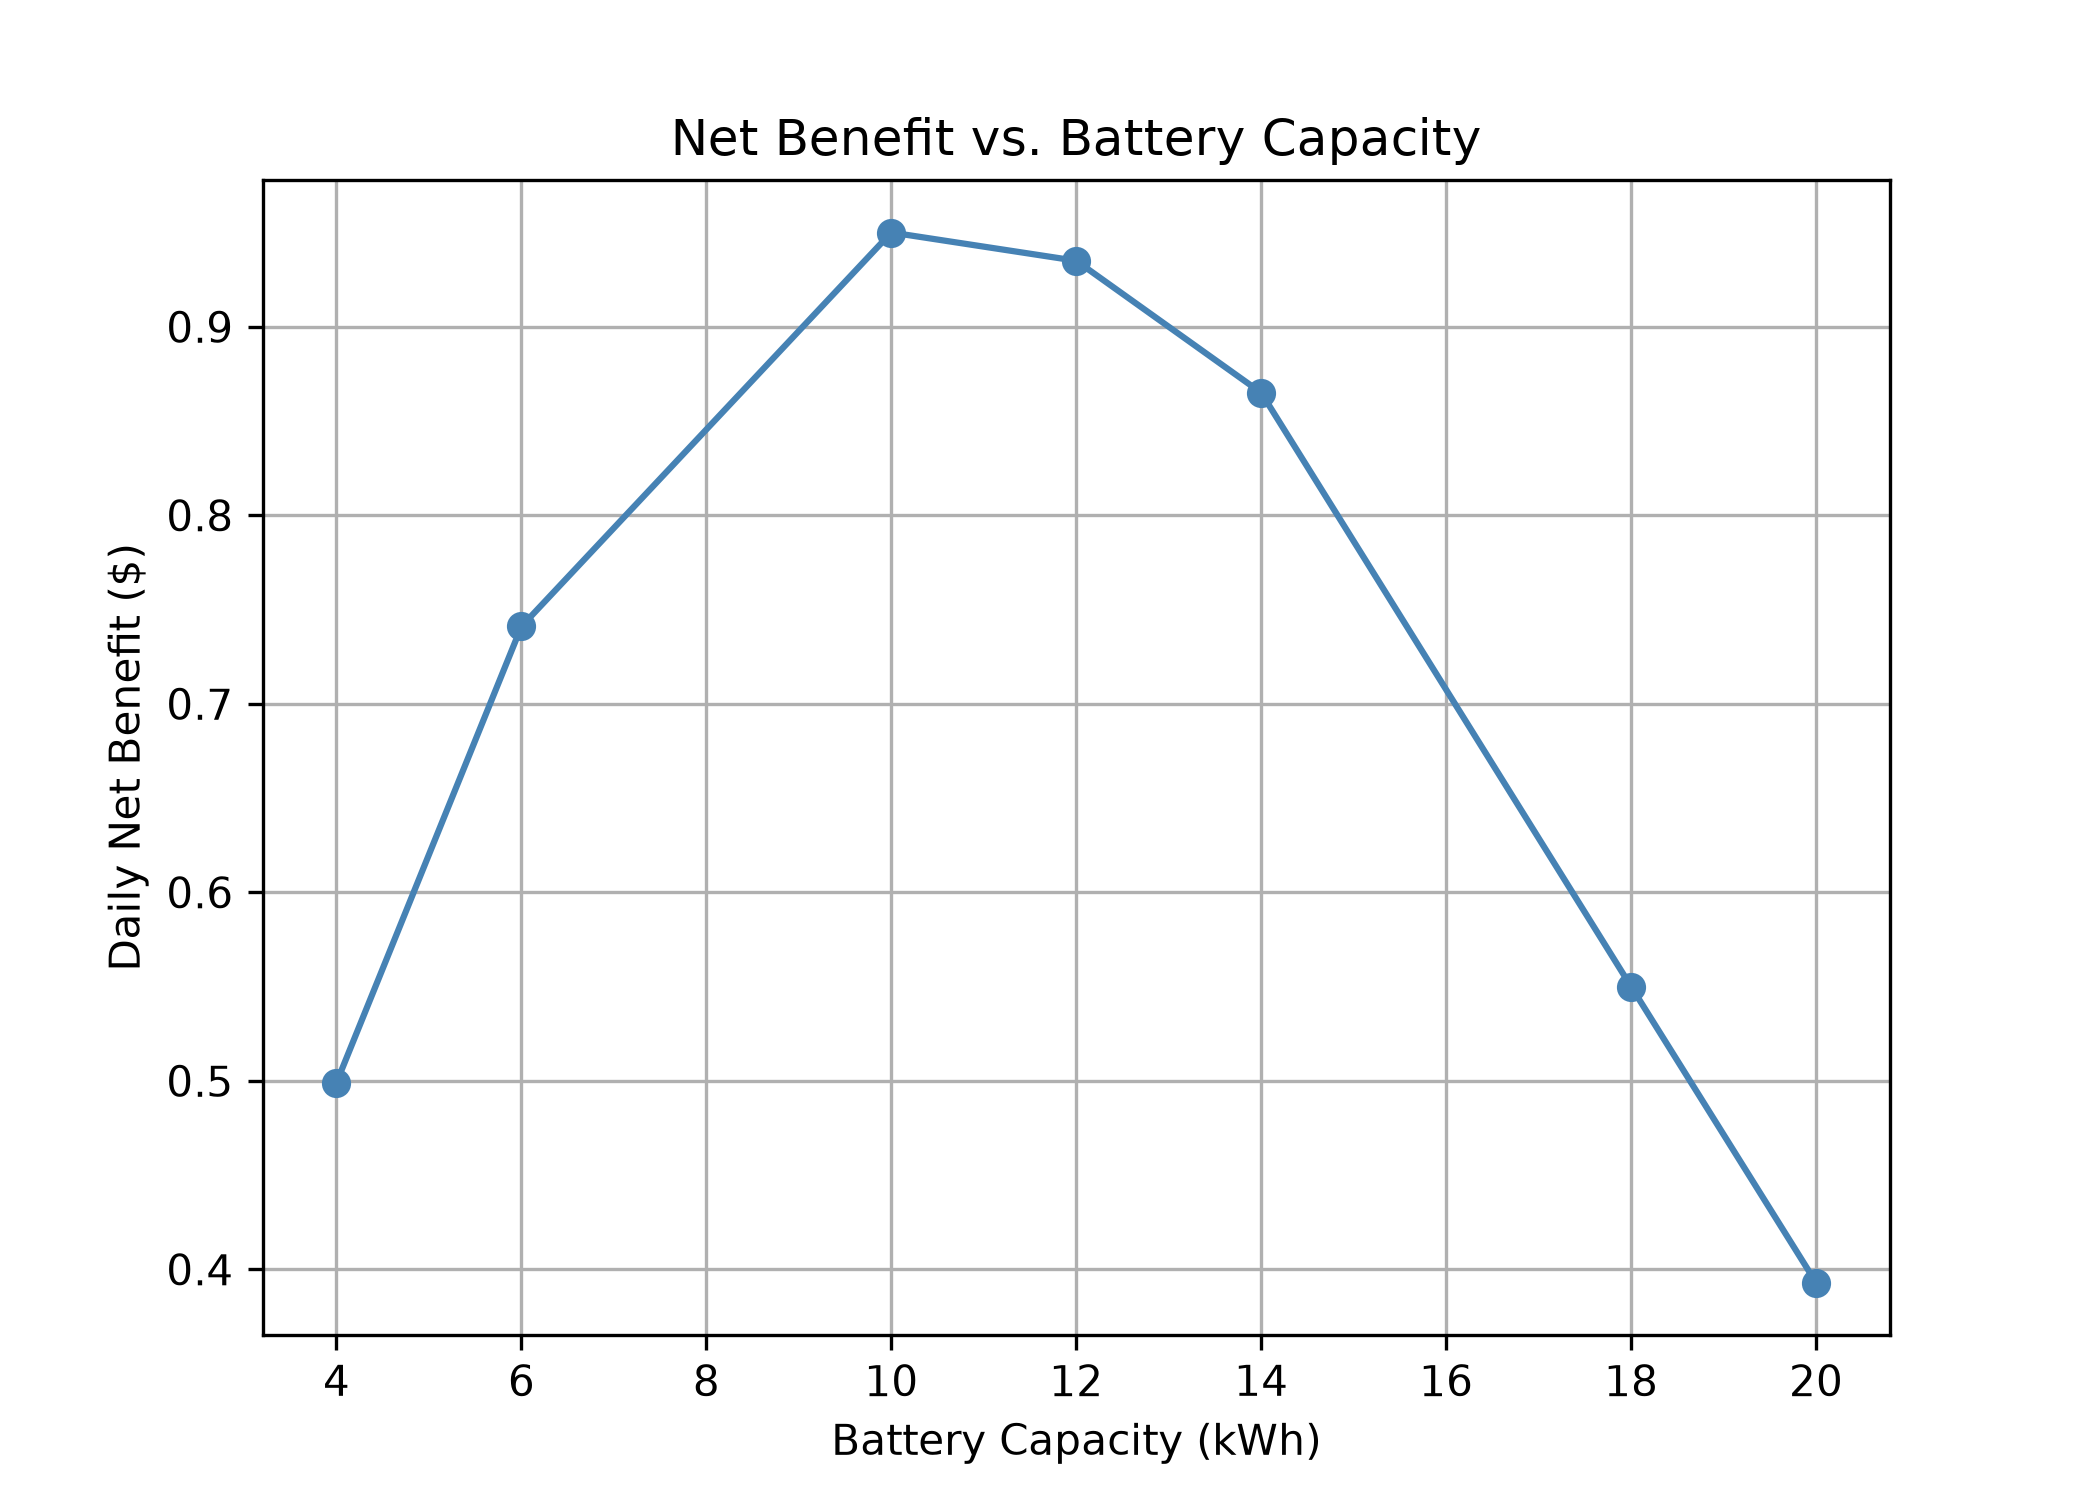
\includegraphics[width=0.5\textwidth]{winter_net_benefit_vs_capacity.png}
    \caption{Winter Net Benefit vs. Battery Capacity}
    \label{fig:winter_net_benefit_image}
\end{figure}

For the summer profile, the highest daily net benefit (\$1.95/day) was achieved with a battery capacity of 12 kWh, although the 14 kWh battery produced a nearly identical net benefit of \$1.94/day. For winter months, the highest daily net benefit (\$0.95/day) was achieved with a battery capacity of 10 kWh. Larger battery capacities did not result in higher net benefits, as the additional capital costs outweighed the incremental operating savings. 

\section{Discussion}
The higher summer net benefit is primarily attributable to greater solar energy production, which allows the battery to store more excess photovoltaic generation during the day and discharge it during higher-priced evening periods. Additionally, NEM 3.0 is structured so that export credits during late summer afternoons can often exceed retail import rates. As a result, homeowners can increase the economic value of their PV-battery system by strategically storing excess solar energy and exporting or using it when electricity costs are highest.  

Furthermore, Fig. 5 and 6 both display how intermediate battery sizes had higher net benefits compared to smaller or larger battery sizes in the range between 4 kWh and 20 kWh. This suggests that although larger batteries can achieve greater electricity bill savings, their annualized capital costs increase more rapidly than the additional savings they provide. For smaller batteries, they are unable to generate enough solar to have the bill savings offset the capital costs. 

The seasonal solar generation, time-of-use pricing, and export credit rates had a significant impact on the affordability of colocation for homeowners in the San Diego region. This was visible in the differences between results for the summer and winter months in the bill savings, operating cost, and net benefit. In all three of these metrics, summer months had a greater value due to both the TOU pricing and export rates being much higher in the summer, allowing homeowners to save and earn more through PV-battery systems. Since solar generation was higher in summer months, there was more solar energy to supply household demand and be transported back to the grid in exchange for export credits. 

It is worth noting that the residential load and solar generation profiles were representative profiles for summer and winter months, so they may not capture any day-to-day variability. Also, the model was only ran seven times for battery capacities (kWh) of 4, 6, 10, 12, 14, 18, and 20. These sizes are considerably spread out, there could be the possibility that the true economically optimal battery size is between two of the evaluated values. 

In the future, this cost minimization model could be applied to a greater range of locations for case studies. We chose San Diego, California for its high electricity prices and solar potential, but it may be valuable to examine states like Nevada where electricity prices are much lower but the solar potential is similar. Additionally, further research avenues could investigate the impact of operation and maintenance costs on the net savings. These costs were not included in this model because they were deemed insignificant compared to the battery's capital costs. 

The findings of this study can help homeowners make more informed battery sizing decisions and provide a foundation for future studies evaluating the economic feasibility of residential PV-battery systems under time-of-use pricing across different seasons and geographic regions.\bibliography{references}


\end{document}
